%%\documentclass[a4paper,12pt,oneside]{llncs}
\documentclass[12pt,letterpaper]{article}
\usepackage[right=2cm,left=3cm,top=2cm,bottom=2cm,headsep=0cm]{geometry}

%%%%%%%%%%%%%%%%%%%%%%%%%%%%%%%%%%%%%%%%%%%%%%%%%%%%%%%%%%%
%% Juego de caracteres usado en el archivo fuente: UTF-8
\usepackage{ucs}
\usepackage[utf8x]{inputenc}

%%%%%%%%%%%%%%%%%%%%%%%%%%%%%%%%%%%%%%%%%%%%%%%%%%%%%%%%%%%
%% Juego de caracteres usado en la salida dvi
%% Otra posibilidad: \usepackage{t1enc}
\usepackage[T1]{fontenc}

%%%%%%%%%%%%%%%%%%%%%%%%%%%%%%%%%%%%%%%%%%%%%%%%%%%%%%%%%%%
%% Ajusta maergenes para a4
%\usepackage{a4wide}

%%%%%%%%%%%%%%%%%%%%%%%%%%%%%%%%%%%%%%%%%%%%%%%%%%%%%%%%%%%
%% Uso fuente postscript times, para que los ps y pdf queden y pequeños...
\usepackage{times}

%%%%%%%%%%%%%%%%%%%%%%%%%%%%%%%%%%%%%%%%%%%%%%%%%%%%%%%%%%%
%% Posibilidad de hipertexto (especialmente en pdf)
%\usepackage{hyperref}
\usepackage[bookmarks = true, colorlinks=true, linkcolor = black, citecolor = black, menucolor = black, urlcolor = black]{hyperref}

%%%%%%%%%%%%%%%%%%%%%%%%%%%%%%%%%%%%%%%%%%%%%%%%%%%%%%%%%%%
%% Graficos 
\usepackage{graphics,graphicx}

%%%%%%%%%%%%%%%%%%%%%%%%%%%%%%%%%%%%%%%%%%%%%%%%%%%%%%%%%%%
%% Ciertos caracteres "raros"...
\usepackage{latexsym}

%%%%%%%%%%%%%%%%%%%%%%%%%%%%%%%%%%%%%%%%%%%%%%%%%%%%%%%%%%%
%% Matematicas aun más fuertes (american math dociety)
\usepackage{amsmath}

%%%%%%%%%%%%%%%%%%%%%%%%%%%%%%%%%%%%%%%%%%%%%%%%%%%%%%%%%%%
\usepackage{multirow} % para las tablas
\usepackage[spanish,es-tabla]{babel}

%%%%%%%%%%%%%%%%%%%%%%%%%%%%%%%%%%%%%%%%%%%%%%%%%%%%%%%%%%%
%% Fuentes matematicas lo mas compatibles posibles con postscript (times)
%% (Esto no funciona para todos los simbolos pero reduce mucho el tamaño del
%% pdf si hay muchas matamaticas....
\usepackage{mathptm}

%%% VARIOS:
%\usepackage{slashbox}
\usepackage{verbatim}
\usepackage{array}
\usepackage{listings}
\usepackage{multirow}

%% MARCA DE AGUA
%% Este package de "draft copy" NO funciona con pdflatex
%%\usepackage{draftcopy}
%% Este package de "draft copy" SI funciona con pdflatex
%%%\usepackage{pdfdraftcopy}
%%%%%%%%%%%%%%%%%%%%%%%%%%%%%%%%%%%%%%%%%%%%%%%%%%%%%%%%%%%
%% Indenteacion en español...
\usepackage[spanish]{babel}

\usepackage{listingsutf8}
% Para escribir código en C
% \begin{lstlisting}[language=C]
% #include <stdio.h>
% int main(int argc, char* argv[]) {
% puts("Hola mundo!");
% }
% \end{lstlisting}


\title{Test de interconexión de red Zybo}
\author{Jesús Rodríguez Heras}

\begin{document}
	
	\maketitle
	\begin{abstract} %Poner esto en todas las prácticas de PCTR
		\begin{center}
			En este documento se desarrolla la explicación y uso de un pequeño script que se usará para el test de interconexión entre los dispositivos de la red Zybo. Debe ser ejecutado desde el ordenador central.
		\end{center}
	\end{abstract}
	\thispagestyle{empty}
	\newpage
	
	\tableofcontents
	\newpage
	
	%%\listoftables
	%%\newpage
	
	%%\listoffigures
	%%\newpage
	
	%%%% REAL WORK BEGINS HERE:
	
	%%Configuracion del paquete listings
	\lstset{language=bash, numbers=left, numberstyle=\tiny, numbersep=10pt, firstnumber=1, stepnumber=1, basicstyle=\small\ttfamily, tabsize=2, extendedchars=true, inputencoding=utf8/latin1}

\section{Descripción}
Una vez se han conectado todos los dispositivos al switch como se indicó en el tutorial de creación de una infraestructura de red de placas Zybo, y, estando encendidos todos los dispositivos, necesitamos comprobar que existe conexión entre todos ellos.

Para ello, se ha desarrollado un script en bash, llamado \texttt{Inicio.sh}, que comprueba el estado de conexión de los dispositivos. En este script se pueden definir las tarjetas Zybo que se vayan a usar, con su alias y su dirección IP de red (previamente establecida). Para ello, tendremos que abrir el fichero \texttt{Inicio.sh} con nuestro editor favorito y cambiar las siguientes líneas:
\begin{figure}[h]
	\centering
	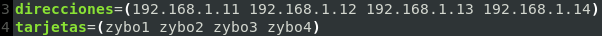
\includegraphics[scale=0.7]{Script.png}
	\caption{Líneas a modificar en el script.}
	\label{Líneas a modificar en el script}
\end{figure}
\begin{itemize}
	\item \textbf{Línea 3:} Introducir la dirección IP de la tarjeta que queramos añadir. O borrar la que queramos quitar.
	\item \textbf{Línea 4:} Introducir el alias de la tarjeta que queramos añadir. O borrar la que queramos quitar.
\end{itemize}

El script será ejecutado desde el ordenador central abriendo una terminal en el directorio donde se ubique el mismo. Cabe destacar que tiene dos modos de funcionamiento:

\subsection{Normal}
En esta opción, la salida del script será meramente informativa, devolviendo si la tarjeta está o no conectada a la red.
\begin{itemize}
	\item Se ejecuta mediante el comando:
	\begin{center}
		\texttt{./Inicio.sh}
	\end{center}
	\item El script lanza cuatro paquetes de ping a cada una de las tarjetas, una por una, guardando el resultado del mismo comando en una variable y sin mostrarla por pantalla.
	\item Mediante scraping\footnote{Técnica usada mediante programas software para extraer información de un texto.} el script lee la salida del último de los paquetes de ping.
	\item \textbf{Éxito:} Si en dicho texto no se encuentra la secuencia ``\texttt{100\% packet loss}'' indicará que la tarjeta está conectada.
	\item \textbf{Fracaso:} Si en dicho texto se encuentra la secuencia ``\texttt{100\% packet loss}'' indicará que la tarjeta a la cual se está realizando el ping, no está conectada.
\end{itemize}

\subsection{Verboso}
En esta opción, la salida del script es más detallada ya que muestra más información al respecto de la conexión.

\begin{itemize}
	\item Se ejecuta mediante el comando:
	\begin{center}
		\texttt{./Inicio.sh -v}
	\end{center}
	\item El script lanza cuatro paquetes de ping a cada una de las tarjetas, una por una.
	\item Mediante la opción \texttt{-v} le indicamos que nos muestre por pantalla la salida de los comandos de ping, para ver el estado de la conexión más detalladamente.
\end{itemize}

\section{Script}
El script está programado en bash y su nombre es \texttt{Inicio.sh}.

\newpage
\subsection{Diagrama de flujo}
\begin{figure}[h]
	\centering
	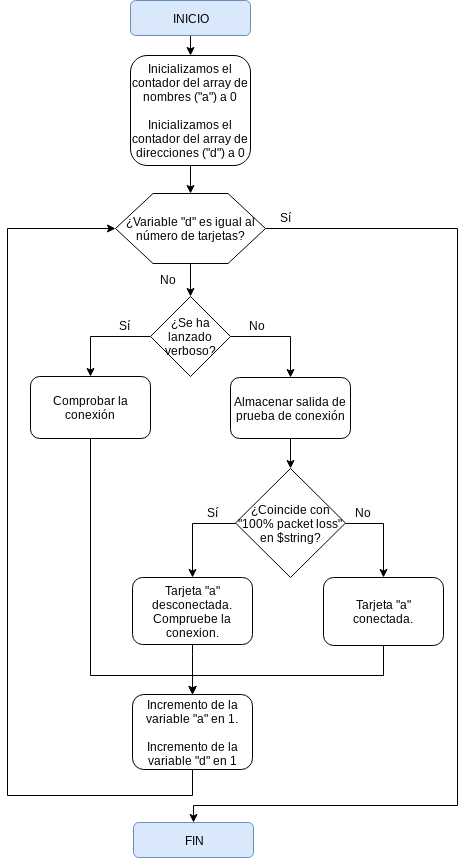
\includegraphics[scale=0.58]{Inicio.png}
	\caption{Diagrama de flujo de \texttt{Inicio.sh}}
	\label{Diagram de flujo de Inicio.sh}
\end{figure}

\newpage
\subsection{Código}
\lstinputlisting[language=Bash]{Inicio.sh}
\begin{center}
	Código de \texttt{Inicio.sh} usando cuatro tarjetas como ejemplo.
\end{center}

\end{document}